
% !TeX root = ../main.tex
\section{Introduction}
\label{sec:introduction}

Balsa (\textit{Ochroma pyramidale}) is a fast-growing tropical tree species whose lightweight wood is widely used as a core material in applications such as wind turbine blades~\citep{Midgley2010Balsa,Jenkin2019BalsaValueChain,Borrega2015Balsa_mechanics}. Ecuador is a major source of commercial balsa, where plantation stands can undergo management-related turnover on cycles of only a few years under productive tropical conditions~\citep{GonzalezOsorio2010Balsa,CanadasLopez2019BalsaGrowth}. Reconstructing these short-rotation dynamics therefore requires a long and temporally continuous observation record capable of resolving multiple disturbance events within the same stand, rather than a single forest-loss label~\citep{CanadasLopez2019BalsaGrowth,Jenkin2019BalsaValueChain}. This requirement is difficult to meet with optical imagery because persistent cloud cover in tropical Ecuador disrupts temporal continuity and can leave critical disturbance periods unobserved. Together, rapid plantation turnover and persistent cloud cover make long-term, cloud-independent SAR observations essential for reconstructing plantation rotation dynamics~\citep{Reiche2018Bayesian,Doblas2020harmonic,Matthew2021BFAST,Bullock2022CCDC_S1,FLORES2026Sensitivity}. The near-decadal Sentinel-1 archive provides the temporal continuity~\citep{Torres2012S1} needed to investigate whether recurrent stand disturbances can be reliably resolved from long-term SAR trajectories.

Long-term plantation management histories have been reconstructed primarily from optical satellite archives. Multi-decadal Landsat records have been used to identify the starts and ends of successive rotations and quantify productivity across thousands of \textit{Eucalyptus} stands~\citep{McMahon2019EucalyptusRotations}, while other time-series approaches have retrieved planting history, harvest timing, generation, rotation length, and stand age in short-rotation plantations~\citep{Du2022GlobalPlantingYears,Li2022EucalyptusHistory}. More recent studies have moved toward denser temporal characterization, including biweekly monitoring of industrial plantation dynamics from PROBA-V~\citep{Bos2025PlantationDynamics} and month-resolved harvest dating and stand-age estimation from Harmonized Landsat--Sentinel imagery~\citep{Huang2026EucalyptusAge}. Sentinel-1 research has developed largely along a complementary trajectory, emphasizing forest disturbance detection and near-real-time warning under cloudy conditions. Dense Sentinel-1 time series have supported probabilistic deforestation monitoring~\citep{Reiche2018Bayesian}, continuous CUSUM-based detection~\citep{RuizRamos2020CUSUMSMC,Ygorra2021CuSum}, selective-logging and plantation-harvest detection~\citep{Matthew2021BFAST,Xulu2020PlantationHarvest}, operational alert systems~\citep{Doblas2022DETERR,Bullock2022CCDC_S1,Mullissa2024LUCA}, and recursive identification of multiple tropical forest disturbances~\citep{Ygorra2023ReCuSum}. Despite these advances, the use of a near-decadal Sentinel-1 record to reconstruct multiple disturbance events within the same managed stand, and thereby recover rotation-relevant histories for a short-rotation plantation system, remains largely unexplored.

Even with dense SAR observations, reconstructing recurrent disturbance events remains challenging. Sentinel-1 backscatter responds not only to canopy structure but also to rainfall and moisture, surface roughness, acquisition geometry, and phenological state, producing temporal variability that can overlap the signal of structural change ~\citep{Doblas2020harmonic,Reiche2018Bayesian,Matthew2021BFAST,vanDerWoude2024S1Disturbance,FLORES2026Sensitivity}. Similar absolute backscatter values may therefore occur under different plantation states, limiting the transferability of a single threshold of backscattering coefficient across stands and environments. After disturbance and subsequent recovery, a fixed historical reference may also cease to represent the current stand condition. CUSUM is feasible because it accumulates persistent departures from an explicit reference state~\citep{Page1954CUSUM}, and Sentinel-1 applications have demonstrated its utility for sustained forest-cover change~\citep{RuizRamos2020CUSUMSMC,Ygorra2021CuSum}. ReCuSum extends this principle to multiple changes through recursive segmentation~\citep{Ygorra2023ReCuSum}, although later segments depend on previously estimated boundaries and may contain progressively fewer observations. For short-rotation plantations, the central methodological challenge is therefore to detect successive disturbances relative to each stand's recent temporal background while maintaining accurate month-level event timing.

These challenges motivate a recurrent-event framework that repeatedly updates each stand's local temporal background as the time series evolves, allowing successive disturbances to be detected relative to the stand's current condition rather than a fixed historical baseline. We therefore propose \textit{Windowed CUSUM}, which implements this principle through overlapping local-reference windows and retains only centrally located negative departures with statistical support before consolidating them into a recurrent disturbance history. This study aims to (1) characterize the within-stand Sentinel-1 response to historical balsa disturbances; (2) evaluate whether Windowed CUSUM improves recurrent-event detection relative to alternative detectors and remains robust to stand representation, polarization, temporal configuration, and statistical assumptions; and (3) reconstruct recurrent plantation disturbance histories and characterize their spatial and temporal dynamics using stand-level event counts and inter-disturbance intervals (Fig.~\ref{fig:national_recurrence_patterns}).
\begin{nolinenumbers}
\begin{figure}[pos=!htbp]
    \centering
    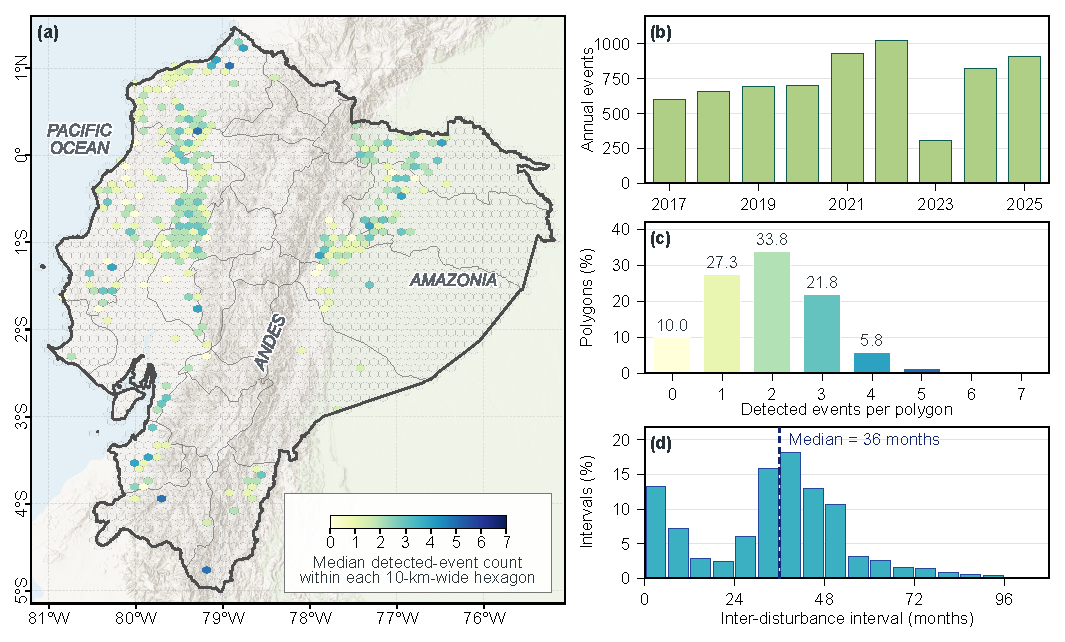
\includegraphics[width=0.92\linewidth]{figures/fig01_national_recurrence.pdf}
    \caption{Recurrent stand-disturbance patterns reconstructed by Windowed CUSUM across the Ecuadorian balsa plantations. (a) Spatial pattern of stand-disturbance recurrence. (b) National annual stand-disturbance frequency. (c) Number of detected disturbances per balsa plantation. (d) Intervals between consecutive detected stand-disturbances; the dashed line indicates the median.}
    \label{fig:national_recurrence_patterns}
\end{figure}
\end{nolinenumbers}




\FloatBarrier
